\documentclass{article}
\usepackage[T1]{fontenc}
\usepackage[unicode]{hyperref}
\usepackage{tikz}
\usepackage{tikzuml/tikz-uml}
\usepackage{graphicx}

\usetikzlibrary{positioning}
\usetikzlibrary{scopes}
\usetikzlibrary{calc}

\title{Zettelkasten GTK}
\author{Kryštof Albrecht \\ \href{mailto:krystofalbrechtus@gmail.com}{krystofalbrechtus@gmail.com}}

\begin{document}
\maketitle
\tableofcontents

\newpage

\section{Introduction}

\subsection{Motivation}

Tools like Vimwiki, Vimzettel and Taskwiki provide a solid base for a Zettelkasten workflow. These are based on \emph{the Vim text editor}, which has a lot of advantages:

\begin{itemize}
	\item Text editing cannot be faster
	
	\item Adding new notes is effortless

	\item The system is simple

	\item Tasks can have note links in them

	\item Any missing functionality can be added through Vimscript
\end{itemize}

The problem is however, that there is no GUI. Tools like \emph{Obsidian} offer a \emph{graph view} that enables natural viewing of the \emph{networked structure} of the Zettelkasten. This view allows faster and easier search and navigation, but also improves the chances of \emph{emergent ideas.}

This tool is based on a \emph{graph view} of the Zettelkasten and allows a wide range of filters to find precisely what we're looking for.

\begin{center}
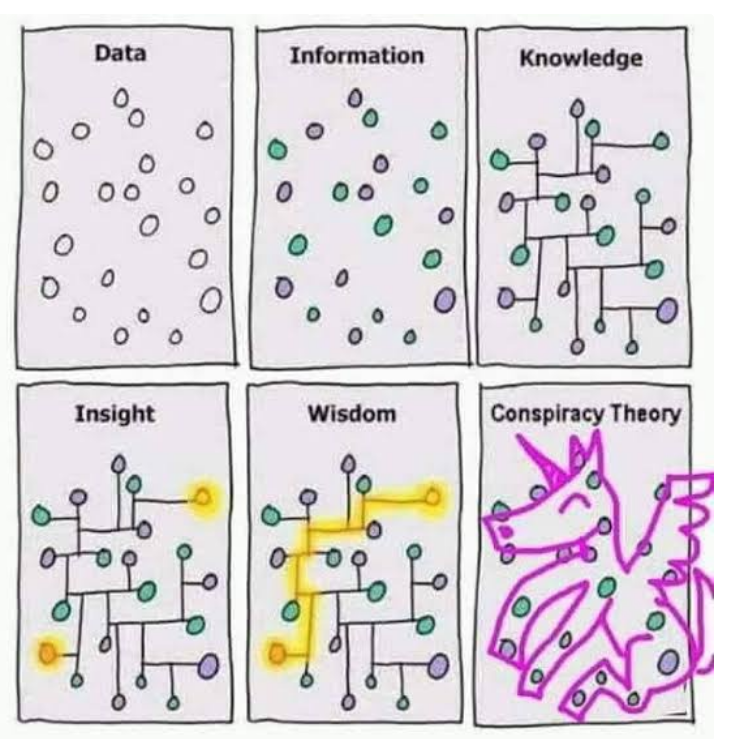
\includegraphics[width=\linewidth/2]{fig/wisdom.png}
\end{center}

\newpage

\subsection{Use case diagram}\label{sec:use_case_diagram}

The graph view (see section \ref{sec:graph_view}) is \emph{the basis} of the system and so will always be shown. The user will then be able to \emph{adjust} this graph view. Any other view will open as a sidebar.

\begin{center}
\begin{tikzpicture}
	\umlactor{User}

	\begin{umlsystem}[x=4]{Zettelkasten GTK}
		\umlusecase[y=1]{Search notes}
		\umlusecase[x=4]{Show result in graph}

		\umlusecase[y=-1]{Show neighboring notes}

		\umlusecase[y=-3]{Show HTML preview}
		\umlusecase[y=-4,x=4]{Highlight hovered link}

		\umlusecase[y=-2]{Open note in Neovim}
		\umlusecase[y=-5,fill=white]{Open calendar/timeline (v2)}
	\end{umlsystem}

	\umlextend{usecase-2}{usecase-1}
	\umlinclude{usecase-4}{usecase-5}

	\umlassoc{User}{usecase-1}
	\umlassoc{User}{usecase-3}
	\umlassoc{User}{usecase-4}
	\umlassoc{User}{usecase-6}
	\umlassoc{User}{usecase-7}
\end{tikzpicture}
\end{center}

\subsection{Miscellaneous features}

Apart from the aforementioned main use cases, there will also be the following features:

\begin{itemize}
	\item Showing files/attachments in the graph view

	\item Support for Vimwiki tags
\end{itemize}

\subsection{Common scenarios}

Here are a few scenarios of how using the application might play out.

\subsubsection{Processing the staging area}

I've taken some notes and put them in the staging area. Now I want to quickly integrate them into the Zettelkasten.

\begin{enumerate}
	\item The staged notes have an \emph{outline} around them in the graph view. Each staging subtask is \emph{further divided} by outlines.

	\item I \emph{highlight} all the task notes within an outline.

	\item I \emph{open} all the notes at once in Neovim with a single click.

	\item I can view the HTML preview of the note I am working on.

	\item As I work, the graph updates \emph{in real time}.
\end{enumerate}

\subsubsection{Searching for information}

I can't seem to remember something that I've written down.

\begin{enumerate}
	\item I enter my search query by \emph{just starting to type.}

	\item The graph updates in real time and shows just the nodes matching the query. The most relevant node is highlighted and its HTML preview is show automatically.

	\item I have the option to show a small snippet of the note next to each node.

	\item Hitting enter, I can navigate the nodes with \emph{Vim keys}.

	\item Hitting enter again, I can navigate the HTML preview.
\end{enumerate}

\newpage

\section{The Graph View}\label{sec:graph_view}

This section provides an overview of the various \emph{elements} of the graph view. 

\begin{center}
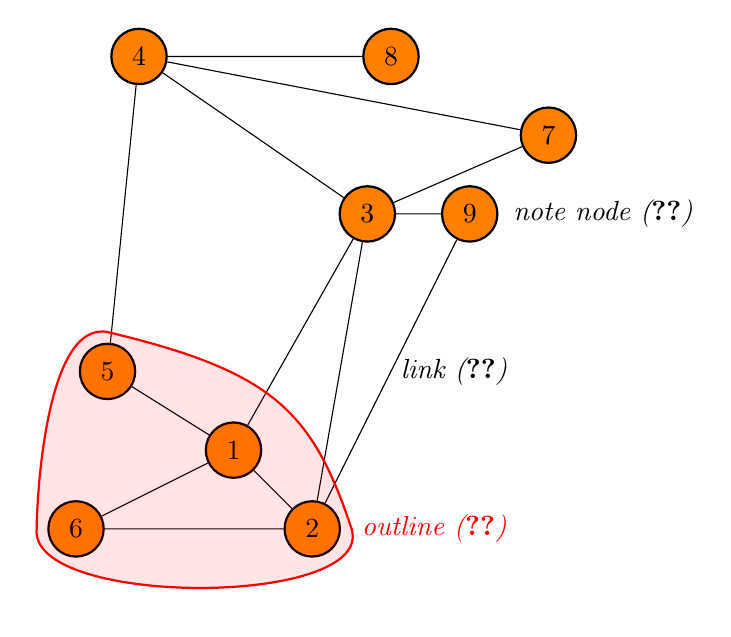
\begin{tikzpicture}
	[note/.style={circle,draw=black,fill=orange,thick,minimum size=2em},
	link/.style={draw=black},
	outline/.style={draw=red,thick}]

	% Draw the graph nodes
	\draw node at (0,0) [note](node1){1} 
		node at (1,-1) [note](node2){2}
		node at (1.7,3) [note](node3){3}
		node at (-1.2,5) [note](node4){4}
		node at (-1.6,1) [note](node5){5}
		node at (-2,-1) [note](node6){6}
		node at (4,4) [note](node7){7}
		node at (2,5) [note](node8){8}
		node at (3,3) [note](node9){9};
	
	% Draw the links between the graph nodes
	\draw[link] (node1) --(node2)
	            (node1) --(node3)
	            (node1) --(node5)
	            (node1) --(node6)
	            (node2) --(node3)
	            (node2) --(node6)
			(node2) -- node[right]{\emph{link (\ref{gelement:links})}}(node9)
			(node3) --(node4)
			(node3) --(node7)
			(node3) --(node9)
			(node4) --(node5)
			(node4) --(node7)
			(node4) --(node8);

		\draw node at ($(node9) + (1.7,0)$){\emph{note node (\ref{gelement:notes})}};

	% Draw outline
		\draw[outline,fill=red,fill opacity=0.1] ($(node5) + (0,0.5)$) .. controls($(node1) + (0.5,1)$) and ($(node1) + (1,0.5)$) .. ($(node2) + (0.5,0)$)

			node[right,red,fill opacity=1]{\emph{outline (\ref{gelement:outlines})}}

			.. controls($(node2) + (0.8,-1)$) and ($(node6) + (-0.6,-1)$) .. ($(node6) - (0.5,0)$)

			.. controls($(node6) + (135:0.7)$) and ($(node5) + (140:1)$) .. ($(node5) + (0,0.5)$);
\end{tikzpicture}
\end{center}

\subsection{Notes}\label{gelement:notes}

\subsection{Links}\label{gelement:links}

\subsection{Outlines}\label{gelement:outlines}

\subsection{Lenses}\label{gelement:lenses}

\end{document}
